\documentclass{beamer}
\usetheme{Madrid}
\usepackage{graphics}

\begin{document}
\title{Game of Life 2D}
\author{Federica Amato, Andrea Bonandin}
\date{21 February 2017}

\begin{frame}
	\begin{center}
		\Large{University of Pavia \\
		Advanced Computer Architecture}
	\end{center}
	\titlepage
\end{frame}

\section{Conway's Game of Life}
\begin{frame}
	\frametitle{Conway's Game of Life}

	\begin{columns}
		\column{0.8\textwidth}
		\begin{block}{Introduction}
			\begin{itemize}
				\item 2-dimensional cellular automaton
				\item Zero-player game
				\item Possibility to create several patterns
				\item States of a population: $0 \rightarrow dead$, $1 \rightarrow alive$
			\end{itemize}
		\end{block}
	\end{columns}
\end{frame}

\section{Transition Rules}
\begin{frame}
	\frametitle{Conway's Game of Life - Transition Rules}
	\begin{itemize}
		\item With zero or one bordering member alive in a cell's neighborhood, death occurs due to loneliness;
		\item With two or three members alive in the neighborhood, there is no change to an alive member;
		\item If a dead member's neighborhood consists of three live members, a new member is born ($0 \rightarrow 1$);
		\item If a live member's neighborhood consists of more than three live members, it will die due to overpopulation.
	\end{itemize}
\end{frame}

\section{Serial Code Analysis}
\begin{frame}
	\frametitle{Serial Code Analysis}
	\begin{itemize}
		\item The universe of the Game is represented by a rectangular grid
		\item Toroidal boundary conditions to reduce errors at the edges
		\item Matrices transformed in 1-D array
	\end{itemize}

	\begin{columns}
		\column{0.9\textwidth}
		\begin{block}{Core functions}
			\textit{init}: it initializes the grid of the Game and the boundaries\\[0.15 cm]
			\textit{evolve}: it updates boundary conditions and applies transition rules\\[0.15 cm]
			\textit{update}: it swaps the previous state with the one
		\end{block}
	\end{columns}
\end{frame}

\section{Serial code Analysis}
\begin{frame}
	\frametitle{\emph{evolve} function}
\end{frame}

\section{OpenMP Parallel Implementation}
\begin{frame}[fragile]
	\frametitle{OpenMP Parallel Implementation}

	\begin{columns}
		\column{0.9\textwidth}
		\begin{block}{Versions}
			\begin{itemize}
				\item \emph{parallel1.c}: one parallel region in every parallelized function, static scheduling
				\item \emph{parallel2.c}: only one parallel region, static scheduling
				\item \emph{parallel3.c}: one parallel region, dynamic scheduling
			\end{itemize}
		\end{block}
	\end{columns}

	\vfill
	We parallelized \emph{for} loops with the directives \begin{semiverbatim}#pragma omp parallel for\end{semiverbatim} \begin{semiverbatim}#pragma omp for\end{semiverbatim}
\end{frame}

\section{Performance's Measurements}
\begin{frame}
	\frametitle{Performance's Measurements}

	\begin{figure}
		\centering
		\begin{minipage}{0.5\textwidth}
			\centering
			\includegraphics[width=\linewidth]{../report/graph.eps}
			\caption{$1000$ generations, $1000x1000$ grid}
		\end{minipage}%
		\begin{minipage}{0.5\textwidth}
			\centering
			\includegraphics[width=\linewidth]{../report/1000-10000.eps}
			\caption{$10000$ generations, $1000x1000$ grid}
		\end{minipage}
	\end{figure}
\end{frame}

\section{Performance's Measurements}
\begin{frame}
	\frametitle{Performance's Measurements}

	\begin{figure}
		\centering
		\begin{minipage}{0.5\textwidth}
			\centering
			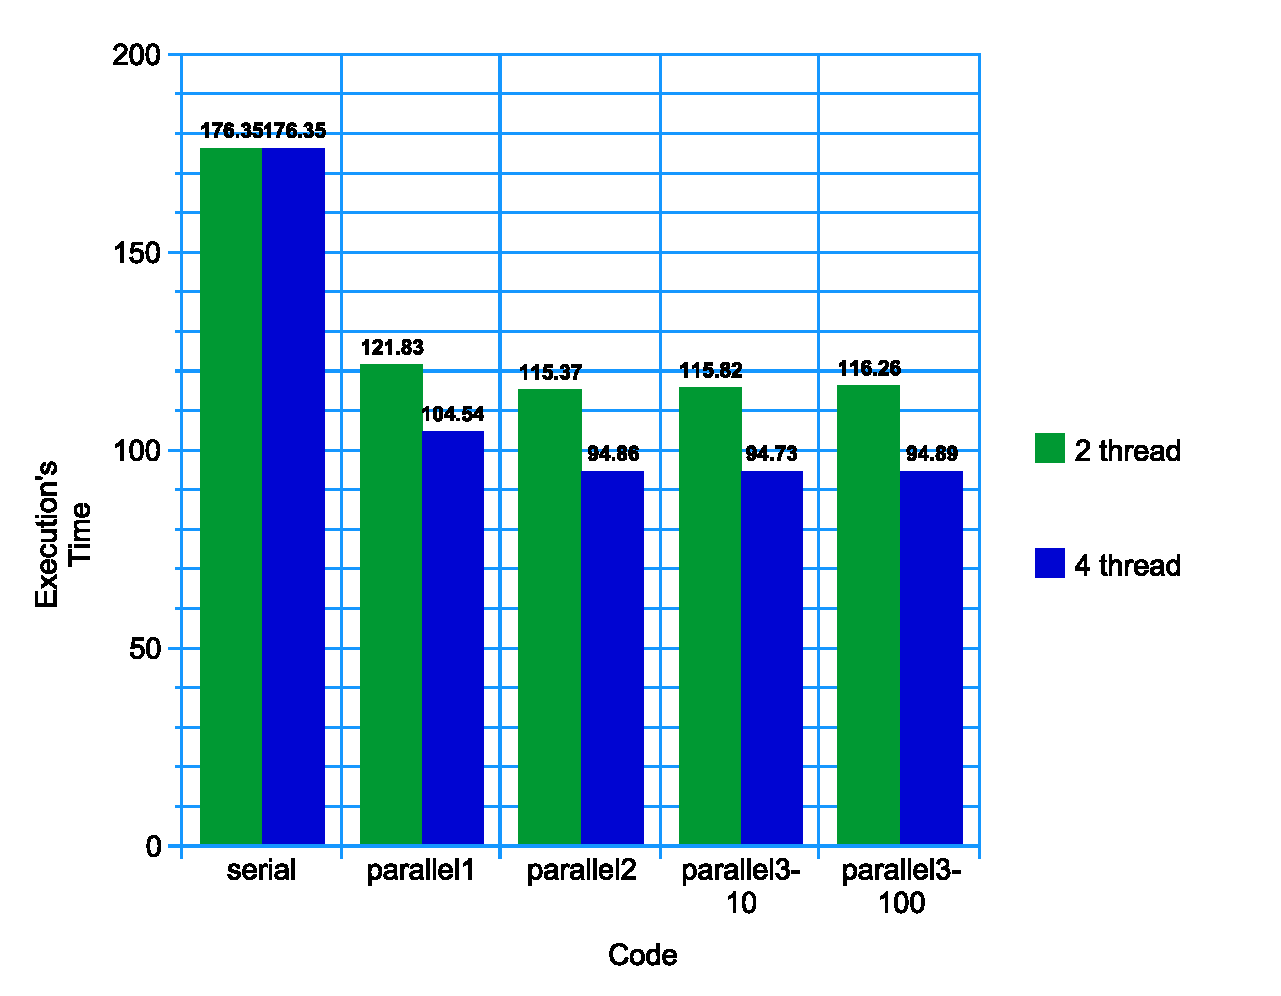
\includegraphics[width=\linewidth]{../report/10000-100.eps}
			\caption{$100$ generations, $10000x10000$ grid}
		\end{minipage}%
		\begin{minipage}{0.5\textwidth}
			\centering
			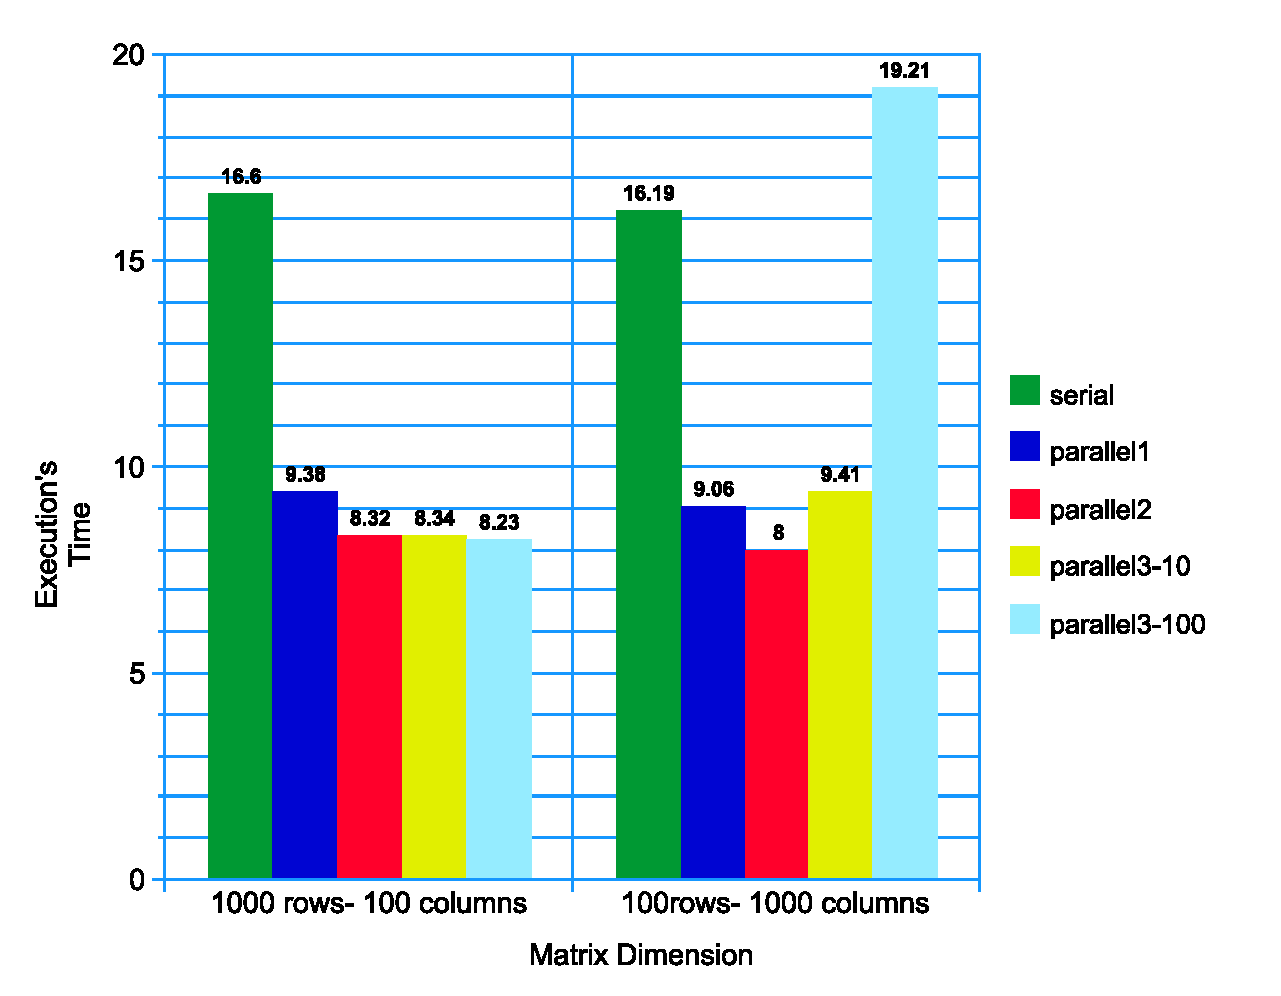
\includegraphics[width=\linewidth]{../report/matdim.eps}
			\caption{$1000$ generations, rectangular grid}
		\end{minipage}
	\end{figure}
\end{frame}

\section{Speedup}
\begin{frame}
	\frametitle{Speedup}

	\begin{figure}
		\centering
		\begin{minipage}{0.5\textwidth}
			\centering
			\includegraphics[width=\linewidth]{../report/2.eps}
			\caption{Speedup with 2 threads}
		\end{minipage}%
		\begin{minipage}{0.5\textwidth}
			\centering
			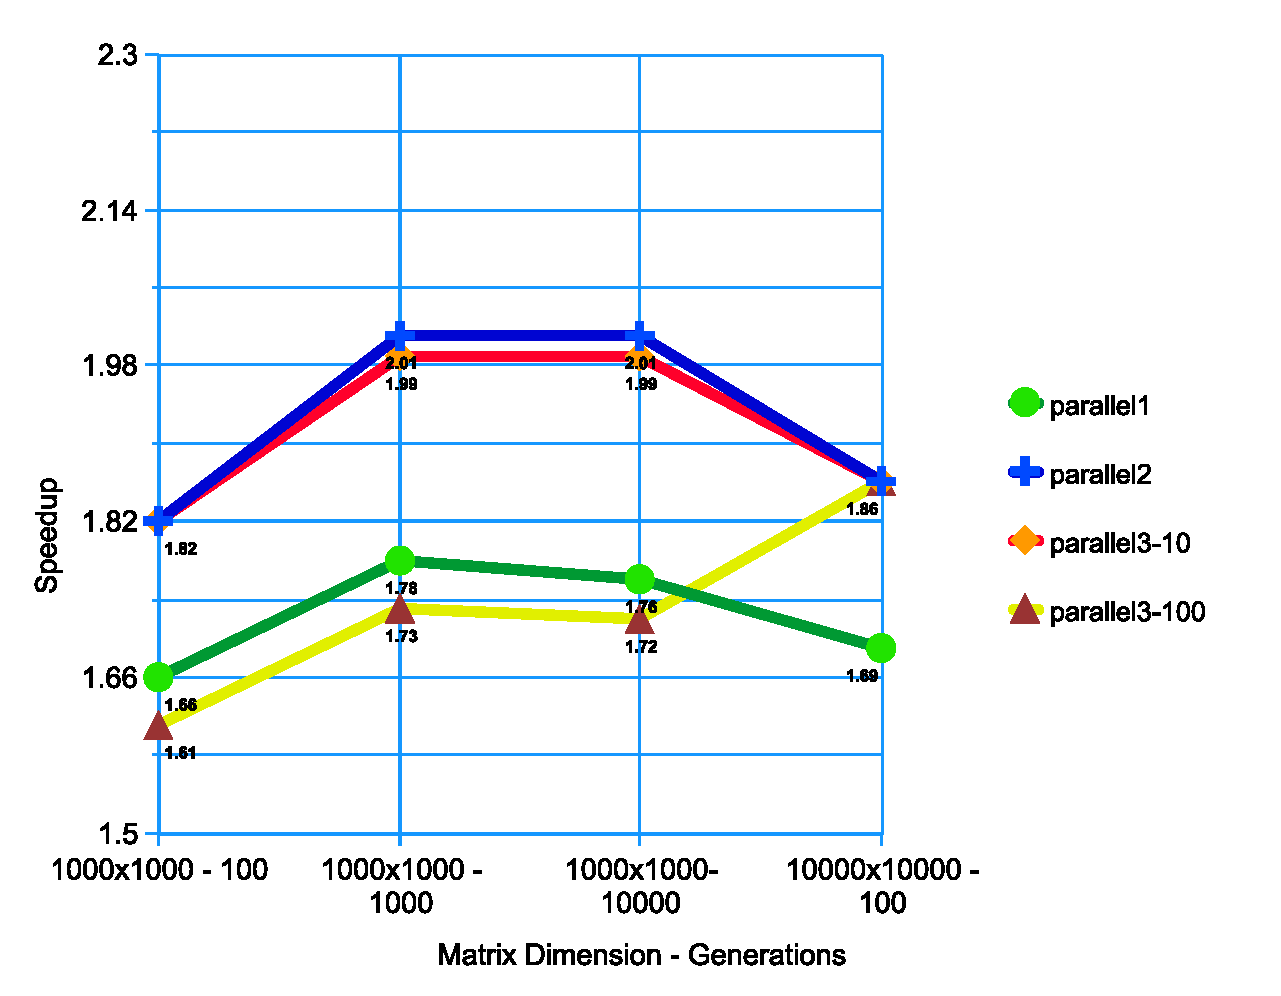
\includegraphics[width=\linewidth]{../report/4.eps}
			\caption{Speedup with 4 threads}
		\end{minipage}
	\end{figure}
\end{frame}

\end{document}
